\chapter{}
As I piloted the Shelby south on I-75, the events of the last 5 days replayed in my mind:
The storm, the park, and Monique. A lot of Monique.

Every once in a while, I'd look over at her, she had fallen asleep about an hour into the
trip home, and was still leaned against the door. I couldn't hear her soft snoring over the
rumble of the big engine, but I knew the sound. Yes, I knew it well.

Last night had been unexpected, but it had been fantastic. She was very loving and
passionate. I have never been with a woman who seemed to put as much of herself into lovemaking
before. It truly had been beautiful. Waking up next to her was great, too. Watching and
listening to her sleep until she woke up, and watching her walk to the bathroom naked except for
the pink cast on her left leg.

We were headed home, and there was a lot to deal with once there. There was the issue of
the damaged house- the repairmen would hopefully be started by now. I also had to get some new
transportation, since the only vehicles I had left were an antique muscle car and a motorcycle.
And then, there were two other women to think about. Two women who were expecting to come and
earn money next week. I wondered how Monique would feel about them. Honestly, I didn't really
care if I casted them or not. They were both very attractive, and casting them had been
enjoyable, but with the relationship developing with Monique, (wow, that was something I
wouldn't have expected to say a week ago!) casting Erin or Samantha wasn't as appealing as it
used to be. Yet, I just wouldn't feel right cutting them off with no warning, not when we had
standing appointments.

\begin{thought}
Monique was dreaming. In her dream, she and Quinn were in Paris, walking along the avenue
in the old town where her father used to do his portraits. In the dream, it was warm, and a
light breeze was blowing. Quinn wore his usual T-shirt and jeans, she wore white linen
drawstring pants and a light blue shell top. She was showing him the areas she frequented when
she lived there. As she told him of her memories at each stop, she was speaking French, and he
was answering in French. She felt very contented, walking hand in hand with Quinn in the
afternoon sun, sharing her early life with him. She awoke to find that they had stopped at a gas
station. Quinn was setting the parking brake, and opening the door.
\end{thought}

``I'm sorry I dozed off on you,'' she said. ``Where are we?''

``That's OK, you're good company even when you're asleep. We're almost to Cincinnati.''

``Wow, that's a long way'', she said, as she got out of the car, stood up, and stretched.

She excused herself, and headed toward the restroom. I watched her walk away, with her
slight limp from the cast on her left leg. She'd wanted to keep it until we got home, and I was
happy to oblige, though she'd had her left leg in one cast or another for most of the last five
days. We couldn't keep her casted all the time, as there was muscle atrophy and other medical
complications that were possible. I met up with her inside, and slipped my arm around her waist
as we went to the register to pay.

The rest of the trip home, she stayed awake, and we talked. We talked about a lot of
things. We had a lot to share with one another, and we just took turns talking about our lives
before we'd met. One of us would say something that sparked a memory in the other one, and a new
area of the conversation would open.

We arrived home shortly after 6:00pm. The storm that had changed our lives so dramatically
had affected the town equally as strong, but where it had been positive for us, it had been
negative for the town: once large trees were now cut back to nothing but trunks, their fallen
branches cut up on the ground beside them. Many houses had their roofs covered with tarpaulins,
and far too many houses had serious damage, or were nothing more than piles of rubble.

As I neared the house, I could see that my (our?) roof was entirely covered with a tarp. As
I turned the corner, I saw a dumpster in the driveway, but there was enough room to get into the
garage. We parked, and a quick peek into the dumpster told me that the repairs were under way-
the dumpster was full of old shingles and guttering.

That evening, I brought up the issue of Erin and Samantha. I really wasn't sure how she'd
take it, but her response had not been all that surprising.

``Quinn, you had an agreement with those women before 'we' happened. If you broke the
agreement with no warning, I'd think less of you.''

I just shook my head and smiled at her. ``You know you're amazing, don't you?''

She cocked her head, raised her eyebrows and said sarcastically ``Yes, but keep telling me,
I like to hear it.'' Then she broke into a smile. Then she took a more serious tone.

``I feel totally at ease with you. I've never trusted anyone much, but with you, it's just
natural. Besides, I know how professional you are.''

At that point, I had an idea.

``Monique, if you'd like, you can help me out with the casting sessions.''

She thought about that a bit. ``That might be fun,'' she said. ``I might have a little cast
envy, but it might still be fun.''

``Speaking of casts, we probably ought to get you out of that one,'' I said, pointing to her
left foot.

She didn't seem thrilled about getting rid of the cast, but we headed for the casting room,
and I cut it off. She walked around a bit to work out some of the stiffness.

Thursday, we went vehicle shopping. We'd left a lot of things undone when we'd taken off
for Ohio and she'd discovered that the shop where her car had been was leveled, and her Firebird
had been destroyed. We were both without everyday transportation. She had planned to take some
of the money from the weekend of the storm and find something used, but I had a different idea.
I needed a pickup truck, but it wasn't always the best vehicle for publicking. We decided that
in addition to a pickup truck, I'd also get a SUV, which would serve well for public cast
adventures, and she could use it to get back and forth to work and school, once it started
again.

When we got home from the dealership, I saw the roofers there, and after talking to them a
bit, they assured me they would be done by Friday afternoon, or Saturday if it rained. Thursday
night, I called Erin and Samantha. I spoke to Erin, and she told me she'd gotten her new cast on
Monday. She said the doctor told her she was healing well, but that she still couldn't go to a
cast below the knee. The good news, she informed me was that they'd given her a cast with her
knee straighter, and it had a walking heel, so she was finally walking without crutches, and was
happy to be rid of them.

When I called Samantha, I got her voice mail, so I left a message stating that I would be
ready the following Wednesday, and asking her to return the call to confirm.

I realized that my stock of supplies was dwindling. I'd used a lot of fiberglass in the
last week- I'd made Erin's body cast and thumb spica, Monique's huge hip and shoulder spica, a
couple of leg casts, and a double shoulder spica. I decided to make a run Friday to get some
more fiberglass and padding. Considering where things were at with Monique, and her preferences,
I also planned to get a good bit of plaster, too.

I invited Monique along, but she was scheduled to work during the day. We'd had a
discussion about her working. She really didn't have to work, but she insisted on paying for her
schooling. She also said that she'd send some of the money to her mother to help out. Of course,
money was nothing to me, but she didn't want me to pay her way for everything. I couldn't talk
her out of it, so I settled for providing living expenses.

\begin{thought}
Friday, after work, Monique returned home, grabbed a quick shower, and put on shorts and a
T- shirt. She really didn't know when to expect Quinn, but she tidied up around the house a bit
while waiting for him. In the front room, she saw the radio they'd used Friday during the storm.
Seeing it reminded her of how intense the day had been, She'd been truly frightened by the
storm, but at the same time, she'd been thrilled to be with Quinn, and to be in such a huge
cast. She put the radio back into the closet she'd seen him get the radio from, and she had a
strange thought- there had been a flashlight there, and they'd taken it downstairs when they'd
gone for shelter from the storm. She was pretty sure they'd left it there, and went to go get
it.

She flipped the light switch, and headed downstairs, remembering Friday. She looked around
the room where they'd taken refuge. She hadn't paid attention then, but she now saw there were a
couple of doors. Curiously, she opened the first door, and saw that it led to a larger room that
was mostly full of boxes. She went to the second door, and opened it. Inside was the furnace and
water heater. On the far wall was another door. A part of her almost felt like she was prying,
looking around like this, but she wasn't opening boxes, only doors. This door led to a sort of
pantry that was probably put there for cool storage when the house was built, as refrigeration
in those days was not what it now was. However, there was no food in this room. What WAS in this
room surprised Monique. The room was filled with removed casts!!

The collection of plaster and fiberglass intrigued her. She picked up a purple long arm
cast and looked at it. It had been carefully removed, and she remembered Quinn had removed her
casts carefully. She looked at it, and at the top of the cast, on the inside, were black
letters. They gave a date of earlier that year, and also the name ``Angie.''

She looked through the rest of the collection. There were nearly thirty cutoff casts in the
room. There was plaster and fiberglass, legs, arms, bodies, and her favorites- the ones with her
name written inside them. She recalled each of them as she picked them up and looked at them.
Out of curiosity, she slipped her leg into one of the long leg casts she'd worn. Of course, it
fit perfectly.

She had an idea.
\end{thought}

As I headed home with a truckload of plaster, fiberglass and padding, my cell phone rang.

``Hi, how far away are you?'' It was Monique.

``I'm about a half hour away. Why do you ask?''

``Would you mind picking up some cigarettes for me? She asked. ``I didn't realize I was low
until I was out of the shower.''

``Sure, I'll see you soon.''

\begin{thought}
``A half hour, that's enough time, if I work fast.'' Monique thought to herself. She got to
work.
\end{thought}

I walked in the back door, and there was no sign of Monique. She wasn't in the kitchen, and
the television wasn't on.

``Monique!''

``In here,'' came a voice from the direction of the setup hospital room.

I walked in and saw something I was absolutely NOT expecting. Monique was lying on the
hospital bed. She had raised the head of the bed slightly, her legs were in the slings, and were
in plaster long leg casts. She was also in a cast from her hips to her neck!

The look on my face must have been amusing, as she broke into a smile.

I noticed that the casts had cut marks, and had been taped together. I realized that they
were casts she had worn before.

``I found these downstairs, and thought I might surprise you,'' she said.

``It worked.''

``I see.''

She lowered the head of the bed with the remote, held up her right hand and used her index
finger to beckon me over.

I went.

\newpage
\begin{center}
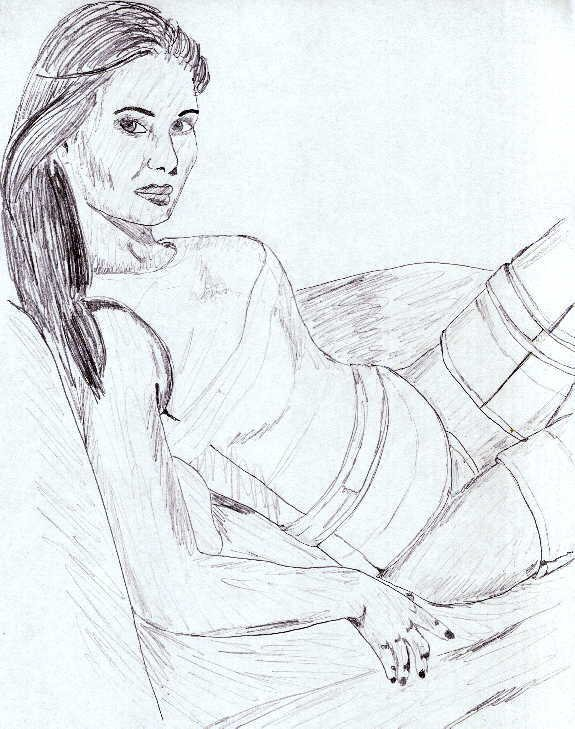
\includegraphics{images/kicks32.jpg}
\end{center}
